\section{Level 1}\label{l1}

\subsection{Entrance}\label{l1:out}

\begin{itemize}
  \item Steep, \textbf{rocky hillside} leads to entrance.
  \item Entrance obscured by\textbf{ vines and thorny bushes}.
  \item Large, \textbf{ominous-looking stones} arranged above entrance.
  \item Foreboding atmosphere causes unease for potential entrants.
  \item \textbf{Sounds:} Rustling of leaves and branches, faint dripping of water.
  \item \textbf{Odors:} Damp earth and decaying vegetation, with a faint hint of something metallic or sulfurous.
\end{itemize}


\subsection{1 : Cobweb Chamber}\label{l1:r1}
\begin{itemize}
  \item Large and dimly lit room \textbf{(30' $\times$ 25' $\times$ 8')}
  \item \textbf{Rough stone walls}, low ceiling
  \item The air is thick with \textbf{dust} and \textbf{cobwebs}
  \item Several \textbf{rat carcasses} littering the floor
  \item A stone \textbf{pedestal} in the center of the room
  \begin{itemize}
    \item Tarnished \textbf{bronze key} sits on top
  \end{itemize}
  \item 1 \textbf{\nameref{monster:spider}} hidden in the ceiling
  \item \textbf{Pressure plate} hidden near the pedestal
  \begin{itemize}
    \item \textbf{Poisonous darts} from hidden vents in the walls
%    \begin{itemize}
      \item 1D4 damage, save vs death cancels; +
      \item 1D4 (poison) save vs poison cancels
%    \end{itemize}
  \end{itemize}
  \item Small \textbf{Narrow tunnel} to the west (5' large).
  Almost hidden.
  \item \textbf{Broad archway} to the east, \textbf{feels cooler}
\end{itemize}

\subsection{2 : "Empty" room}\label{l1:r2}
\begin{itemize}
  \item Narrow tunnel leads \textbf{downwards}.
  \item Opens up into a \textbf{small, roughly ovoid chamber} (\textbf{10' $\times$ 10' $\times$ 5'}).
  \item The walls and floor are rough and uneven.
  \item Smell of \textbf{damp earth} and \textbf{rotting wood}.
  \item \textbf{Hidden} under debris : small \textbf{brass button} set into the stone floor
  \begin{itemize}
    \item Stone wall slides back if pushed
    \item Reveals hidden chamber
  \end{itemize}
\end{itemize}

\subsection{3 : Hidden chamber}\label{l1:r3}
\begin{itemize}
  \item \textbf{15' $\times$ 20' $\times$ 10'}
  \item The walls are made of rough-hewn stone
  \item The floor is covered in a layer of dust
  \item A single torch sputters on the wall, casting flickering shadows across the room.
  \item A \textbf{large stone pedestal} in the center
  \begin{itemize}
    \item A beautiful \textbf{golden chalice} (500 GP)
    \item If taken :
    \begin{itemize}
      \item Room begins to shake violently
      \item Floor opens to a pit filled with spikes
      \item 2D6 damages (save vs death : \textonehalf)
    \end{itemize}
  \end{itemize}
\end{itemize}

\vfill
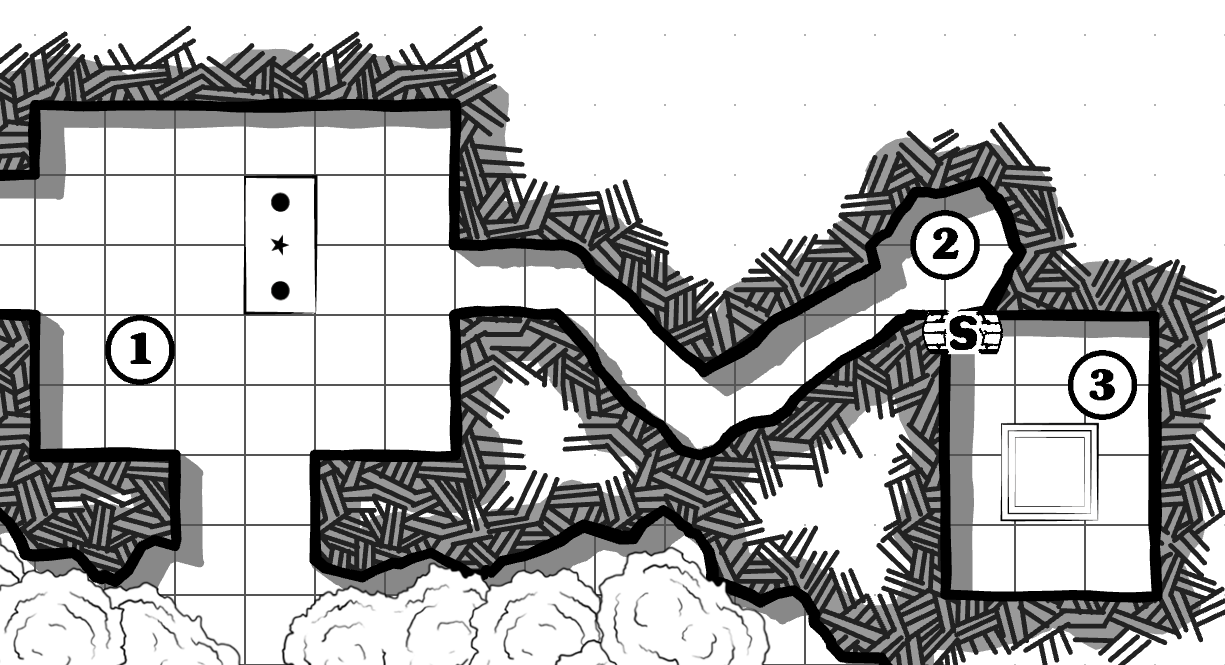
\includegraphics[width=\linewidth]{pics/map_1-3.png}

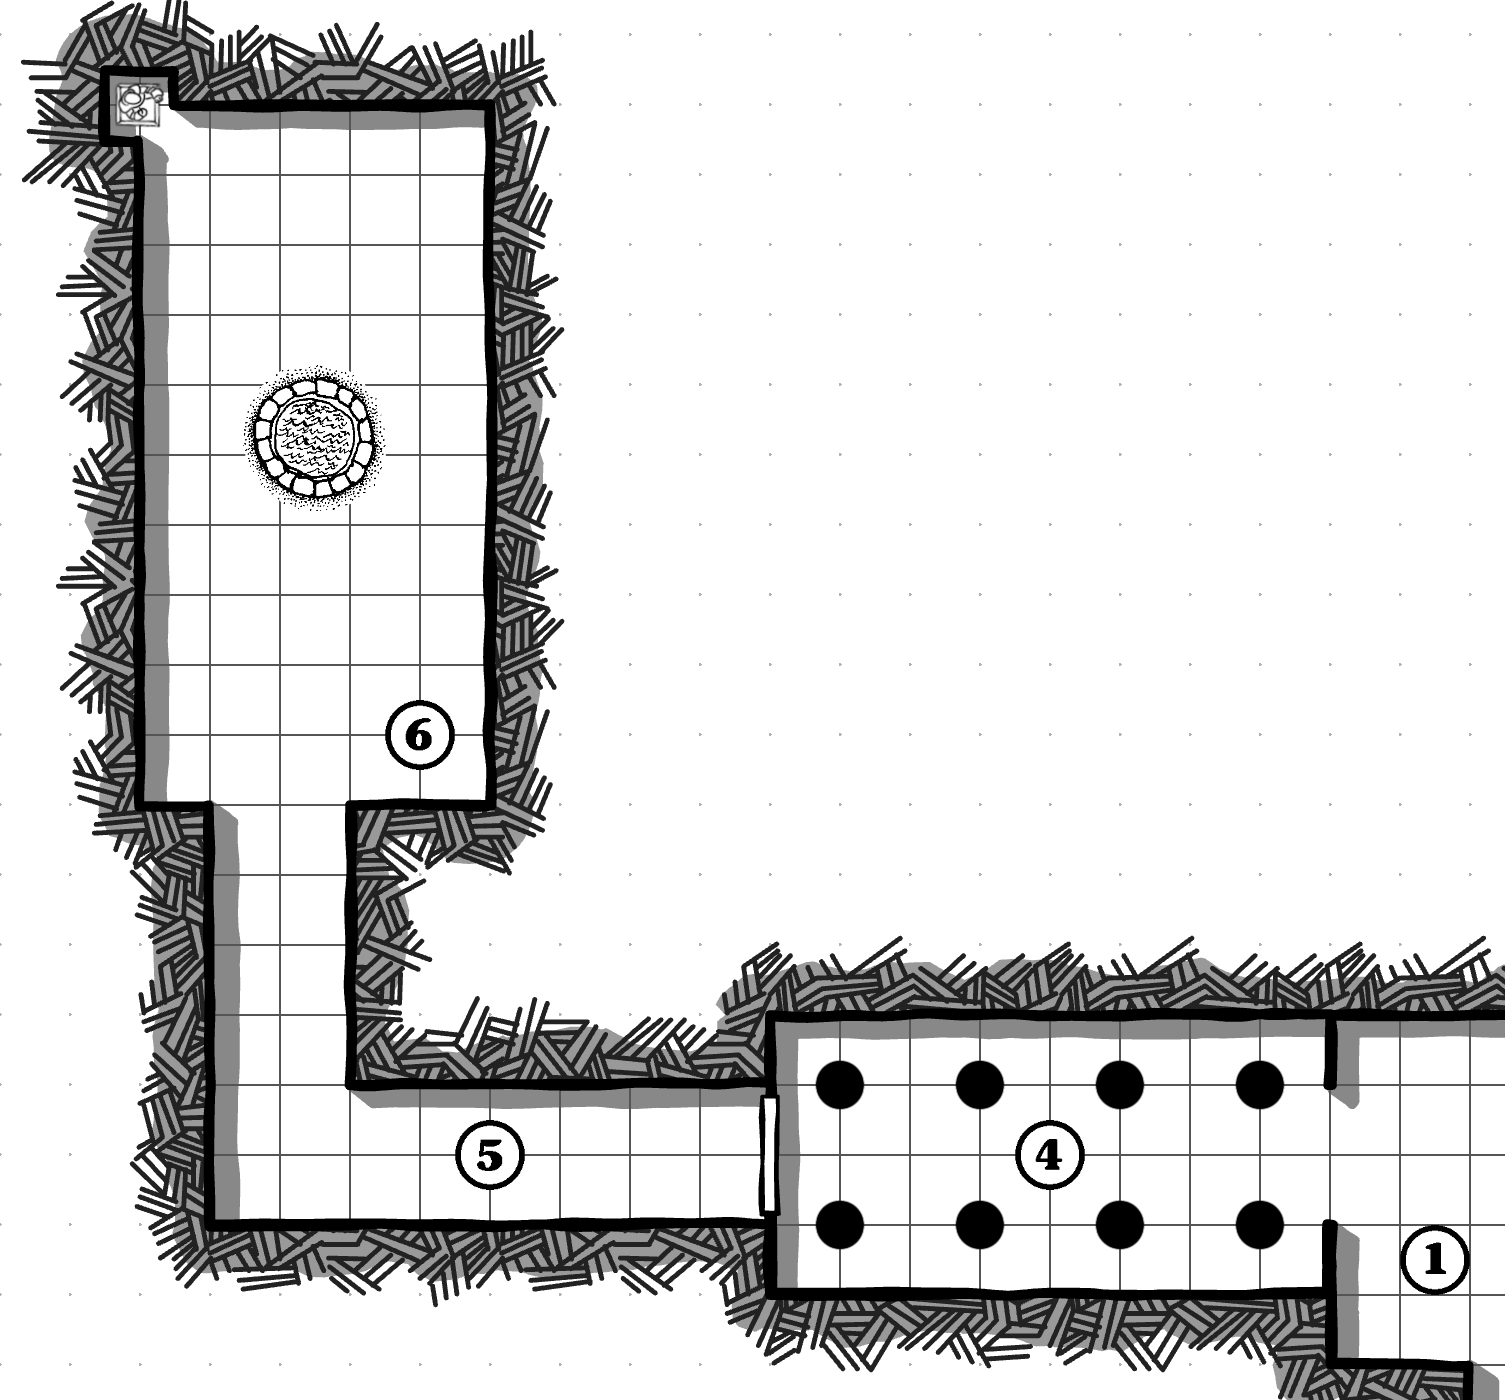
\includegraphics[width=\linewidth]{pics/map_4-6.png}
\subsection{4 : Hall of Echoes}\label{l1:r4}
\begin{itemize}
  \item Long corridor \textbf{20' $\times$ 40' $\times$ 10'}
  \item The walls are made of rough-hewn stone.
  \item 2 rows of 4 columns.
  \begin{itemize}
    \item Scenes of \textbf{battle} and \textbf{conquest}
    \item Scenes of people worshipping a \textbf{shadowy figure} (details obscured by darkness)
  \end{itemize}
  \item Any sound is amplified by echo :
    alerts monsters from \textbf{\nameref{l1:r6}}
  \item \textbf{Strange mosaic} on the floor :
  \begin{itemize}
    \item A serpent wrapped around a sword
    \item \textbf{Message} written in an unknown language
    \begin{highlight}
      \emph{"Beware the artifact of shadows, for its power consumes all who seek to possess it."}
    \end{highlight}
  \end{itemize}
  \item Far end : \textbf{stone door}
  \begin{itemize}
    \item Intricate carvings
    \begin{itemize}
      \item Same \textbf{shadowy figure} with elongated limbs and sharp claws
      \item Worshippers offering sacrifices
      \item Eyes glowing with an otherworldly energy
      \item Inspires darkness, fear, and death
    \end{itemize}
    \item Locked (bronze key)
  \end{itemize}
\end{itemize}

\subsection{5 : Low corridor}\label{l1:r5}
\begin{itemize}
    \item \textbf{30' + 30' $\times$ 10' $\times$ 6'}
    \item Roughly hewn out of stone
    \item Straight for 30' before turning right
    \item \textbf{Low ceiling}, forcing to crouch slightly
    \item Dim blue light source in the distance
\end{itemize}

\subsection{6 : The Chamber of Radiance}\label{l1:r6}
\begin{itemize}
    \item \textbf{30' $\times$ 40' $\times$ 15'}
    \item \textbf{Glowing crystals} embedded in the walls and ceiling : soft blue light.
    \item Circular \textbf{pool of water} at center (10' $\diameter$).
    \begin{itemize}
        \item Calm and clear
        \item Glowing faintly from within
        \item \textbf{Big crystal} at the bottom of the pool
        \item Embedded in a ovoid transparent stone (1000 GP)
        \item Guarded by a \textbf{\nameref{monster:specter}} bound to the pool
        \item Crystal powers the \textbf{\nameref{monster:specter}}:
        \begin{itemize}
            \item Source of "life power"
            \item Without the Crystal the \textbf{\nameref{monster:specter}} suffers :
            +2 THACO ; -4 AC ; $\textonehalf$ HP.
        \end{itemize}
    \end{itemize}
    \item Same carving as in \textbf{\nameref{l1:r4}}
    \item N-W : alcove -- \textbf{statue of the shadowy god}.
    \begin{itemize}
        \item made of black stone
        \item 7' tall
        \item Its hand closed around a missing item
        \item \textbf{Message} (same unknown language) : \emph{"Drinking power"}
    \end{itemize}
    \item 3d4 \textbf{\nameref{monster:skeleton}}, 1 \textbf{\nameref{monster:ghoul}}
    \item No visible other exits from the chamber
\end{itemize}

\begin{highlight}[To \nameref{l2}]
    \begin{itemize}
        \item Place the ovoid stone containing the big crystal inside the chalice from \textbf{\nameref{l1:r3}}
        \item Place this chalice inside the statue's hand
        \item The wall behind the statue slides
        \item The statue slides into the opened area
        \item Reveal stairs to \textbf{\nameref{l2}}
    \end{itemize}
\end{highlight}
